% ==================================================
% فصل ترجمه مقاله Nature
% ==================================================

\chapter{ترجمه فارسی مقاله \textit{Observation of constructive interference at the edge of quantum ergodicity}}
\label{chap:otoc-translation}

% مسیر تصاویر (در صورتی که فایل‌ها در پوشه `figs/` قرار داشته باشند)
\graphicspath{{figs/}}

در این جا، ترجمه‌ای تحلیلی از مقالهٔ جدید گروه \lr{Google Quantum AI} با عنوان «\lr{Observation of constructive interference at the edge of quantum ergodicity}» که در مجلهٔ \lr{Nature} در اکتبر 2025 منتشر شده است ارائه می‌شود \cite{google2025observation}. این مقاله به بررسی دینامیک سیستم‌های چندجسمی کوانتومی با استفاده از توابع همبستگی خارج از ترتیب زمانی \lr{Out-of‑Time‑Order Correlators – OTOC} پرداخته و نشان می‌دهد که اندازه‌گیری‌های مرتبهٔ دوم این تابع، اطلاعاتی را در اختیار قرار می‌دهد که در روش‌های کلاسیکی قابل دسترسی نیستند.

\section{مقدمه و انگیزهٔ پژوهش}

دینامیک سیستم‌های چندجسمی کوانتومی غالباً با همبستگی‌هایی در مکان‌ها و زمان‌های مختلف مشخص می‌شود. در سامانه‌هایی که به سرعت درهم‌تنیده می‌شوند، بیشتر مشاهده‌پذیرهای محلی در زمان‌های طولانی به جزئیات دینامیک حساس نیستند و به بیان ساده، اطلاعات اولیه در فضای هیلبرت وسیع «پخش» یا \lr{scramble} می‌شود. این مسئله باعث می‌شود که اندازه‌گیری‌های متعارف در مدت زمان نسبتاً کوتاهی فروپاشی کرده و نتوانند آشوب کوانتومی و ارگودیسیتی را آشکار کنند.  پژوهشگران برای غلبه بر این محدودیت از پروتکل‌های زمان-معکوس یا «دنبالهٔ اکو» استفاده می‌کنند تا بخش عمدهٔ تکامل را خنثی کرده و سیگنال‌های ظریف را بازیابی کنند.
در این مقاله، تیم \lr{Google Quantum AI} خانواده‌ای از آزمایش‌های \lr{OTOC} را بر روی پردازندهٔ کوانتومی مبتنی بر کیوبیت‌های ابررسانا انجام می‌دهد. آنها با تغییر تعداد بازوهای تداخل (مرتبهٔ \(k\) تابع \lr{OTOC}) و افزودن جابجایی‌های فاز تصادفی یا منسجم، نشان می‌دهند که اندازه‌گیری \lr{OTOC(2)} نسبت به جزئیات میکروسکوپی تکامل بسیار حساس‌تر از همبستگی‌های عادی و مرتبهٔ اول است

\begin{figure}[htbp]
  \centering
  \IfFileExists{figs/fig1.png}{%
    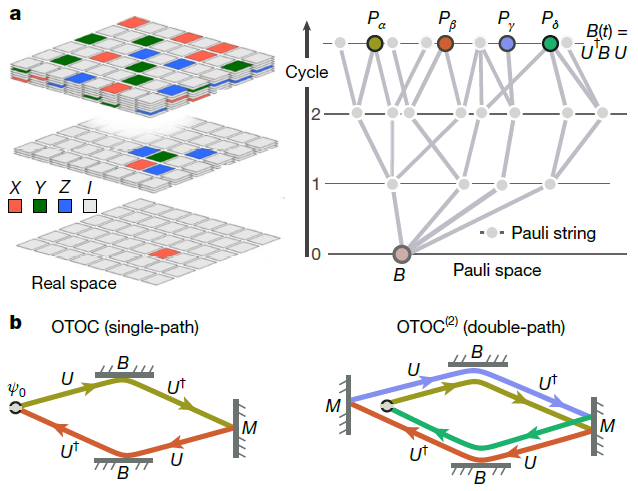
\includegraphics[width=0.85\textwidth]{figs/fig1.png}
  }{%
    \fbox{تصویر 'figs/fig1.pdf' یافت نشد؛ در صورت وجود، آن را در پوشه `figs/` قرار دهید.}
  }
  \caption{ساختار کلی و شماتیکِ پروتکل‌های OTOC (شکل توضیحی). }
  \label{fig:otoc-protocol}
\end{figure}

\section{تعریف و فرمول‌بندی \lr{OTOC}}

فرض کنید دو عملگر کوانتومی \(A\) و \(B\) را داریم. در تصویر هایزنبرگ، عملگر \(A(t)=U^{\dagger}(t)\,A\,U(t)\) با گذر زمان \(t\) تکامل می‌یابد که در آن \(U(t)=e^{-iHt}\) تکامل زمانی تحت همیلتونی \(H\) است. تابع همبستگی خارج از ترتیب زمانی \lr{OTOC} برای این دو عملگر به صورت زیر تعریف می‌شود:
\begin{equation}
  OTOC(t)=\langle A(t)\,B\,A(t)\,B\rangle,
\end{equation}
که در آن \(\langle\cdot\rangle\) میانگین روی حالت اولیهٔ سیستم است. اگر \(A\) و \(B\) در ابتدای زمان جابه‌جایی‌پذیر باشند اما با گذر زمان commute نکنند، مقدار \lr{OTOC} کاهش می‌یابد و این کاهش نشانه‌ای از پخش اطلاعات (اثر پروانه‌ای کوانتومی) است.

پژوهشگران برای دسترسی به اطلاعات دقیق‌تر، از نسخهٔ مرتبهٔ دوم \lr{OTOC(2)} استفاده کردند که با دو بار اجرای پروتکل زمان-معکوس به دست می‌آید. فرمول عمومی \lr{OTOC(k)} به صورت زیر است:
\begin{equation}
  \mathcal{C}_k^{(2)}(t)=\bigl\langle \left[ U^{\dagger}(t)\,B\,U(t)\,M\right]^k \bigr\rangle,
\end{equation}
که در آن \(M\) یک عملگر پائولی (مثلاً \(X\) یا \(Z\)) است و \(k\) تعداد بازوهای تداخل را تعیین می‌کند. برای \(k=2\) داریم
\begin{equation}
  \mathcal{C}_2^{(2)}=\langle U^{\dagger}(t)\,B\,U(t)\,M\,U^{\dagger}(t)\,B\,U(t)\,M\rangle.
\end{equation}
این کمیت همان \lr{OTOC(2)} است و می‌تواند به صورت جمعی از چهار رشتهٔ پائولی در فضای پائولی بازنویسی شود. در صورتی که حاصل ضرب چهار رشته به عملگر یکه منتهی شود، تداخل سازنده رخ می‌دهد و سهم آن مسیر تقویت می‌شود.

\section{پروتکل‌های آزمایشی و حساسیت \lr{OTOC}}

در آزمایش‌های این مقاله، پردازندهٔ کوانتومی شامل شبکه‌ای از کیوبیت‌های ابررسانا است که با گیت‌های تک‌کیوبیتی تصادفی و گیت‌های دوکیوبیتی ثابت اجرا می‌شوند. ابتدا دو کیوبیت مشخص \(q_m\) و \(q_b\) به عنوان محل اعمال عملگرهای \(M\) و \(B\) انتخاب می‌شوند. سپس مدارهای تصادفی مختلف با پارامترهای گیت‌های تک‌کیوبیتی متفاوت تولید شده و برای هر مدار، مقدار \(\mathcal{C}_k^{(2)}\) اندازه‌گیری می‌شود.
. برای کاهش نویز، اندازه‌گیری‌ها آنقدر تکرار می‌شود تا خطای آماری کمتر از ده درصد مقدار میانگین باشد.  در نهایت، تمام مقادیر با عامل مقیاس جهانی که از استراتژی‌های تصحیح خطا بدست می‌آید نرمال‌سازی می‌شوند.
نتایج نشان می‌دهد که \lr{OTOC(2)} (و به طور کلی \lr{OTOC(k)}) نسبت به جزئیات دینامیک کوانتومی حساس است. برای مثال، با اندازه‌گیری \(\mathcal{C}^{(4)}\) برای فواصل مختلف بین \(q_m\) و \(q_b\)، مرز واضحی مشاهده می‌شود که فراتر از آن مقدار \lr{OTOC} تقریباً برابر یک است؛ این مرز همان مخروط نوری کیوبیت \(q_m\) است. علاوه بر این، انحراف معیار \lr{OTOC(2)} در نزدیکی مرز اطلاعات هم‌مرتبه با مقدار متوسط آن است، که بیانگر حساسیت زیاد این تابع به تکامل زیرین است. مقایسه با همبستگی‌های ترتیب زمانی معمول نشان می‌دهد که انحراف معیار \lr{OTOC} به صورت قانون توانی آهسته فرو می‌ریزد، در حالی که همبستگی‌های عادی به سرعت نمایی کاهش می‌یابند.

\begin{figure}[htbp]
  \centering
  \IfFileExists{figs/fig2.png}{%
    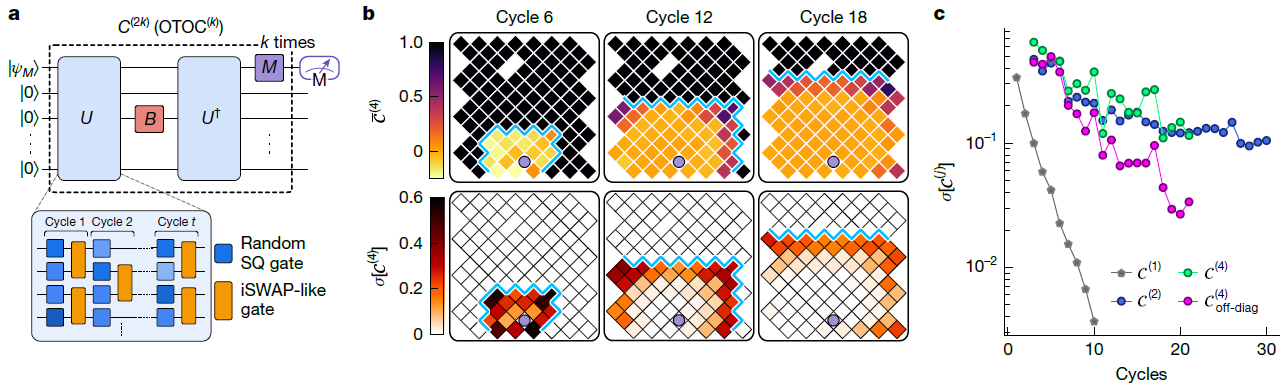
\includegraphics[width=0.8\textwidth]{figs/fig2.png}
  }{%
    \fbox{تصویر 'figs/fig2.pdf' یافت نشد؛ در صورت وجود، آن را در پوشه `figs/` قرار دهید.}
  }
  \caption{حساسیت OTOC به جزئیات میکروسکوپی دینامیک — شکلِ شماتیک/نمونه.}
  \label{fig:otoc-sensitivity}
\end{figure}

\section{تداخل بزرگ و حلقه‌های سازنده در \lr{OTOC(2)}}

در بخش دیگری از آزمایش، پژوهشگران تغییر کوچکی در فاز یکی از بازوهای تداخل ایجاد کردند تا تأثیر تداخل کوانتومی را بررسی کنند. آن‌ها نشان دادند که \lr{OTOC(2)} به این تغییرات فاز بسیار حساس است و این حساسیت به دلیل تداخل سازنده میان مسیرهای مختلف در فضای پائولی است



. در این حالت، ترکیب چهار رشتهٔ پائولی می‌تواند به عملگر یکه منجر شود و بنابراین سیگنال تقویت شود. این نوع تداخل، که به «تداخل حلقهٔ بزرگ» معروف است، در \lr{OTOC(1)} مشاهده نمی‌شود و محاسبهٔ کلاسیکی آن بسیار دشوار است. برای سیستم‌های با ۴۰ تا ۶۵ کیوبیت، شبیه‌سازی دقیق این کمیت با کامپیوترهای کلاسیک به چند سال زمان نیاز دارد، در حالی که پردازندهٔ کوانتومی می‌تواند آن را در چند ساعت اندازه‌گیری کند.

\begin{figure}[htbp]
  \centering
  \IfFileExists{figs/fig3.png}{%
    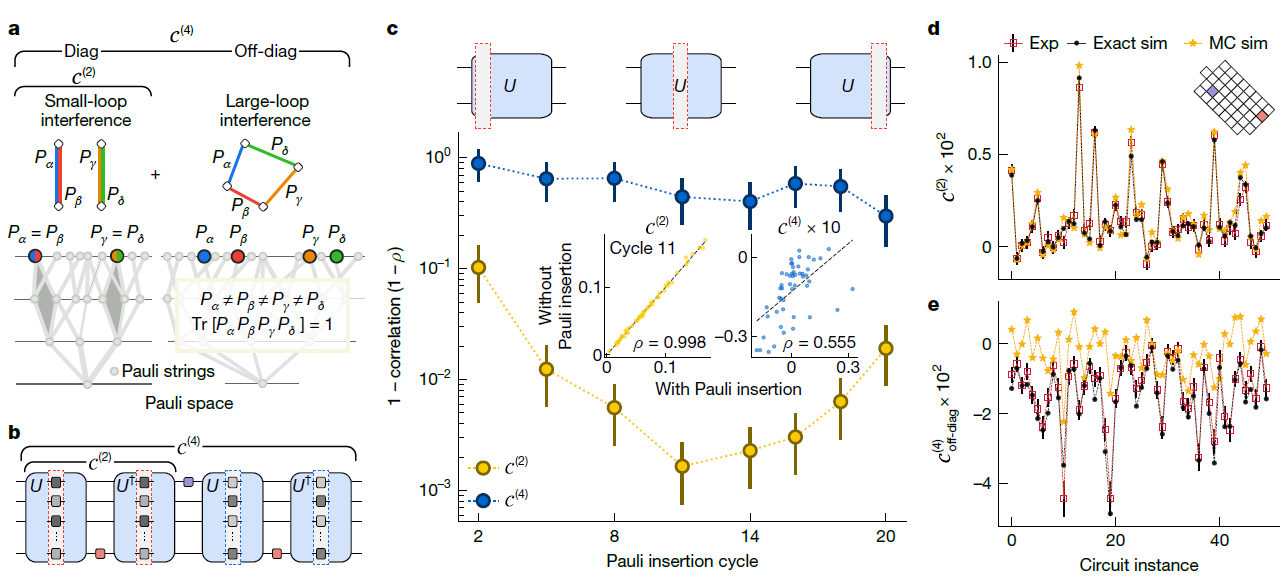
\includegraphics[width=0.75\textwidth]{figs/fig3.png}
  }{%
    \fbox{تصویر 'figs/fig3.pdf' یافت نشد؛ در صورت وجود، آن را در پوشه `figs/` قرار دهید.}
  }
  \caption{نمونه‌ای از «تداخل حلقهٔ بزرگ» که منجر به تقویت سیگنال OTOC می‌شود. }
  \label{fig:otoc-interference}
\end{figure}

\section{کاربرد در یادگیری همیلتونی}

یکی از کاربردهای مهم \lr{OTOC(2)} که در مقاله مورد بررسی قرار گرفته «یادگیری همیلتونی» است. فرض کنید سیستم فیزیکی واقعی دارای همیلتونی مجهولی با چند پارامتر ناشناخته باشد. می‌توان با اندازه‌گیری \lr{OTOC(2)} در این سیستم و مقایسهٔ آن با شبیه‌سازی کوانتومی همان سیستم (که در آن پارامترها متغیر هستند)، مقدار پارامترهای ناشناخته را پیدا کرد. پژوهشگران برای نشان دادن این مفهوم، یک مثال تک‌پارامتری را در نظر گرفتند که در آن فاز \(\xi\) یک گیت دوکیوبیتی ناشناخته است. آنها مجموعه‌ای از داده‌های \(\mathcal{C}_{\text{off-diag}}^{(4)}\) را از ۲۰ مدار تصادفی شبیه‌سازی‌شده به عنوان «داده‌های سیستم فیزیکی» در نظر گرفتند و سپس همان مدارها را روی پردازندهٔ کوانتومی اجرا کردند. با تغییر \(\xi\) و محاسبهٔ اختلاف بین داده‌های تجربی و داده‌های شبیه‌سازی‌شده، نموداری به دست آمد که حداقل آن دقیقاً برابر مقدار واقعی \(\xi\) بود. این آزمایش نشان می‌دهد که \lr{OTOC(2)} می‌تواند به عنوان ابزاری قدرتمند برای تخمین پارامترهای همیلتونی پیچیده استفاده شود.

\begin{figure}[htbp]
  \centering
  \IfFileExists{figs/fig4.png}{%
    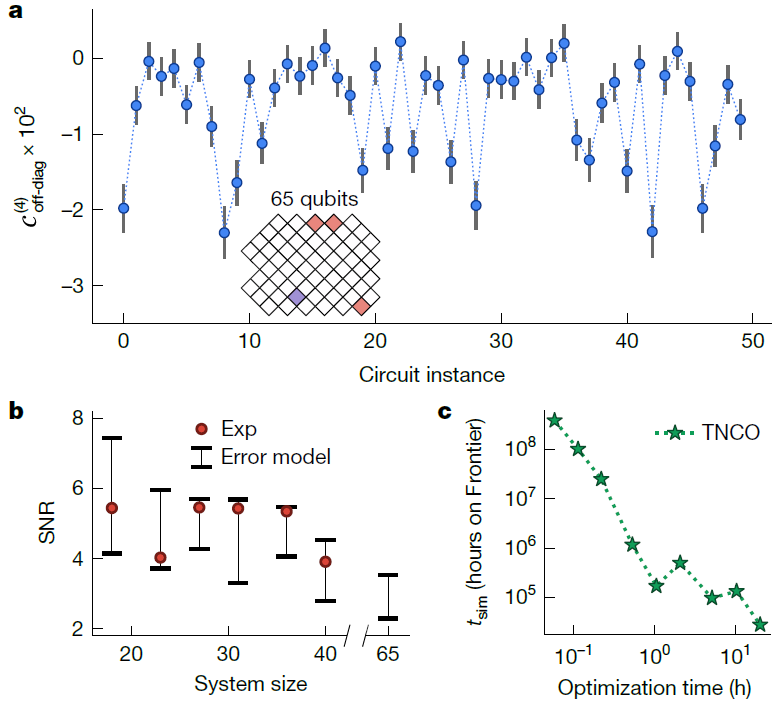
\includegraphics[width=0.8\textwidth]{figs/fig4.png}
  }{%
    \fbox{تصویر 'figs/fig5.pdf' یافت نشد؛ در صورت وجود، آن را در پوشه `figs/` قرار دهید.}
  }
  \caption{نمونه‌ای از روند به‌کارگیری OTOC در یادگیری همیلتونی؛ منحنی اختلاف یا loss بر حسب پارامتر فاز \(\xi\).}
  \label{fig:otoc-hamiltonian-learning}
\end{figure}


\begin{figure}[htbp]
	\centering
	\IfFileExists{figs/fig5.png}{%
		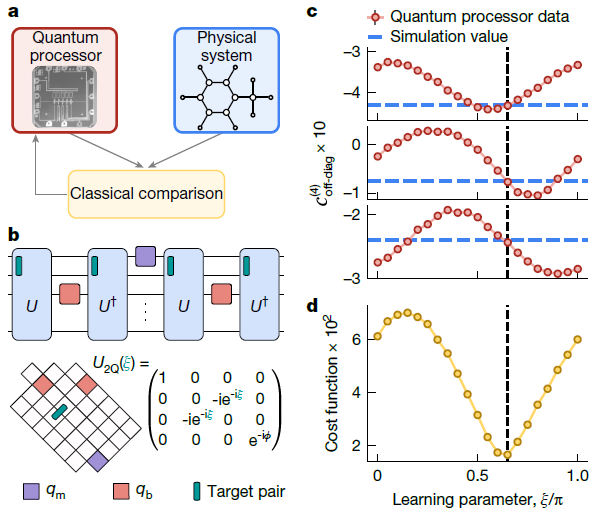
\includegraphics[width=0.8\textwidth]{figs/fig5.png}
	}{%
		\fbox{تصویر 'figs/fig5.pdf' یافت نشد؛ در صورت وجود، آن را در پوشه `figs/` قرار دهید.}
	}
	\caption{نیاز به تکیمل کپشن }
	\label{fig:otoc-hamiltonian-learning}
\end{figure}
\section{مزیت کوانتومی عملیاتی}

مقالهٔ گوگل نشان می‌دهد که \lr{OTOC(2)} نه تنها به پدیده‌های بنیادین مانند آشوب کوانتومی و تداخل سازنده حساس است، بلکه از نظر پیچیدگی محاسباتی در محدوده‌ای قرار دارد که شبیه‌سازی کلاسیکی آن فعلاً امکان‌پذیر نیست. در یک آزمایش، اندازه‌گیری \(\mathcal{C}_{\text{off-diag}}^{(4)}\) برای مدارهای ۶۵ کیوبیتی انجام شد و دقت سیگنال در حد \lr{SNR} بین ۲ تا ۳ باقی ماند

. تخمین زده شد که شبیه‌سازی همین داده‌ها با استفاده از الگوریتم‌های شبکهٔ تانسوری روی ابررایانهٔ \lr{Frontier} حدود ۳.۲ سال زمان می‌برد
، در حالی که اندازه‌گیری آزمایشی تنها ۲.۱ ساعت طول کشید. این اختلاف عظیم، همراه با قابلیت استخراج اطلاعات مفید (مانند یادگیری همیلتونی)، نشان می‌دهد که \lr{OTOC(2)} گزینهٔ مناسبی برای دستیابی به مزیت کوانتومی عملیاتی است.
\section{جمع‌بندی  }

در این فصل ترجمهٔ مختصری از مقالهٔ «مشاهدهٔ تداخل سازنده در لبهٔ ارگودیسیتی کوانتومی» ارائه شد. مقاله نشان می‌دهد که چگونه اندازه‌گیری‌های \lr{OTOC(2)} می‌توانند ساختارهای تداخلی پیچیده و حساسیت بالایی به دینامیک کوانتومی داشته باشند و در عین حال شبیه‌سازی کلاسیکی آن‌ها فوق‌العاده دشوار است. این ویژگی‌ها، همراه با کاربردهای عملی مانند یادگیری همیلتونی، راهی ملموس به سوی مزیت کوانتومی در سیستم‌های واقعی باز می‌کند.

\subsection*{اهمیت مقاله}
این کار اهمیت زیادی دارد چون نشان می‌دهد کمیت‌هایی مانند \lr{OTOC(2)} می‌توانند اطلاعاتی بنیادین دربارهٔ آشوب و پخش اطلاعات در سامانه‌های چندجسمی ارائه دهند که با ابزارهای متعارف قابل دسترسی نیست. همچنین نشان داده شد که اندازه‌گیری‌های انتخاب‌شده روی سخت‌افزار کوانتومی واقعی در مقیاس‌هایی که شبیه‌سازی آن‌ها کلاسیکی دشوار است، عملی و نسبتاً سریع است.

\subsection*{نوآوری‌های کلیدی}
نوآوری‌های اصلی مقاله را می‌توان به طور خلاصه این‌گونه بیان کرد:
\begin{itemize}
  \item معرفی و مطالعهٔ سیستماتیک \lr{OTOC(2)} و کاربرد آن برای آشکارسازی تداخل سازنده در مسیرهای تکاملی مختلف.
  \item طراحی پروتکل‌های زمان-معکوس و استفاده از دستکاری فاز و تعداد بازوهای تداخل برای تقویت سیگنال‌های ظریف کوانتومی.
  \item ارائهٔ شواهد تجربی از محدوده‌ای که در آن اندازه‌گیری‌های خاص روی سخت‌افزار کوانتومی می‌توانند مزیت زمانی نسبت به شبیه‌سازی کلاسیکی داشته باشند (نمونهٔ عملی از مزیت کوانتومی عملیاتی).
\end{itemize}

\subsection*{کاربردهای احتمالی}
نتایج این پژوهش چند کاربرد بالقوه را پیش‌روی پژوهشگران می‌گذارد:
\begin{itemize}
  \item یادگیری همیلتونی: استفاده از \lr{OTOC(2)} به عنوان معیار کمّی برای برازش پارامترهای همیلتونی سامانه‌های چندجسمی که شبیه‌سازی آن‌ها کلاسیکی دشوار است.
  \item تشخیص و تحلیل آشوب کوانتومی و انتقال‌های دینامیکی: حساسیت بالای این کمیت می‌تواند برای شناسایی گذارهای دینامیکی و نقاط بحرانی مفید باشد.
  \item سنجش و اعتبارسنجی سخت‌افزار کوانتومی در مقیاس‌های بزرگ: اندازه‌گیری‌هایی که شبیه‌سازی آن‌ها برای کامپیوترهای کلاسیک زمان‌بر است، می‌تواند معیاری برای سنجش توان حقیقی سیستم باشد.
  \item کاربردهای سنجشی  \lr{(quantum sensing)}: طراحی پروتکل‌هایی که از تداخل سازنده برای تقویت سیگنال‌های ضعیف استفاده کنند.
\end{itemize}

\subsection*{محدودیت‌ها و چشم‌اندازها}
چند محدودیت مهم نیز باید مدنظر باشد: نیاز به کنترل نویز و خطا در گیت‌ها برای مقیاس‌های بزرگ‌تر، وابستگی نتایج به انتخاب دقیق مدارها و عملگرها، و نیاز به آمار زیاد برای کاهش خطای آماری. چشم‌اندازهای آینده شامل بهبود روش‌های تصحیح خطا، بهینه‌سازی طراحی مدارها برای افزایش SNR، و تعمیم مفاهیم به کلاس‌های گسترده‌تر همیلتونی‌ها و نشانه‌ها است.
